\documentclass[11pt,a4paper]{article}

\usepackage[a4paper,top=20mm,bottom=20mm,left=19mm,right=19mm,headheight=15pt]{geometry}
\usepackage[T1]{fontenc}
\usepackage{lmodern}
\usepackage{microtype}
\usepackage{graphicx}
\usepackage{booktabs}
\usepackage{tabularx}
\usepackage{array}
\usepackage{longtable}
\usepackage{amsmath}
\usepackage{enumitem}
\usepackage{xcolor}
\usepackage{fancyhdr}
\usepackage{titlesec}
\usepackage{hyperref}
\usepackage{lastpage}
\usepackage{caption}
\usepackage{float}

\definecolor{Navy}{HTML}{17324D}
\definecolor{Teal}{HTML}{167C80}
\definecolor{PaleTeal}{HTML}{E8F3F3}
\definecolor{PaleBlue}{HTML}{EDF2F7}
\definecolor{Warm}{HTML}{F6F1E8}
\definecolor{Ink}{HTML}{25313C}
\definecolor{Muted}{HTML}{647482}
\definecolor{Rule}{HTML}{CCD6DD}

\hypersetup{
  colorlinks=true,
  linkcolor=Navy,
  urlcolor=Teal,
  pdftitle={Preliminary Motor and Joint-Torque Analysis - ExoEskeleto v1},
  pdfauthor={Engineering analysis prepared from ExoEskeleto Drawing v1}
}

\color{Ink}
\setlength{\parindent}{0pt}
\setlength{\parskip}{5.5pt}
\setlist[itemize]{leftmargin=5mm,itemsep=2pt,topsep=3pt}
\setlist[enumerate]{leftmargin=6mm,itemsep=2pt,topsep=3pt}
\renewcommand{\arraystretch}{1.18}
\captionsetup{font=small,labelfont={bf,color=Navy}}

\titleformat{\section}
  {\Large\bfseries\color{Navy}}
  {\thesection}{0.65em}{}
  [\vspace{-3pt}\color{Teal}\titlerule]
\titleformat{\subsection}
  {\large\bfseries\color{Navy}}
  {\thesubsection}{0.55em}{}
\titleformat{\subsubsection}
  {\normalsize\bfseries\color{Teal}}
  {\thesubsubsection}{0.5em}{}
\titlespacing*{\section}{0pt}{13pt}{7pt}
\titlespacing*{\subsection}{0pt}{10pt}{4pt}
\titlespacing*{\subsubsection}{0pt}{8pt}{3pt}

\pagestyle{fancy}
\fancyhf{}
\fancyfoot[L]{\small\color{Muted}Preliminary engineering analysis}
\fancyfoot[R]{\small\color{Muted}Page \thepage\ of \pageref*{LastPage}}
\renewcommand{\headrulewidth}{0pt}
\renewcommand{\footrulewidth}{0pt}
\fancypagestyle{plain}{%
  \fancyhf{}
  \fancyfoot[L]{\small\color{Muted}Preliminary engineering analysis}
  \fancyfoot[R]{\small\color{Muted}Page \thepage\ of \pageref*{LastPage}}
  \renewcommand{\headrulewidth}{0pt}
  \renewcommand{\footrulewidth}{0pt}
}

\newcommand{\unit}[1]{\ensuremath{\,\mathrm{#1}}}
\newcommand{\Nm}{\unit{N\,m}}
\newcommand{\highlightbox}[2]{%
  \begingroup
  \setlength{\fboxsep}{8pt}%
  \noindent\colorbox{#1}{\parbox{\dimexpr\linewidth-2\fboxsep\relax}{#2}}%
  \endgroup
}
\newcommand{\ratingcard}[3]{%
  \begin{minipage}[t]{0.30\textwidth}
    \colorbox{PaleTeal}{\parbox[c][27mm][c]{\dimexpr\linewidth-2\fboxsep\relax}{
      \centering\color{Navy}\bfseries #1\\[2pt]
      {\Large\color{Teal}#2}\\[-1pt]
      {\scriptsize\color{Muted}#3}
    }}
  \end{minipage}%
}

\begin{document}

\begin{titlepage}
  \thispagestyle{empty}
  \vspace*{-5mm}
  {\color{Teal}\rule{\linewidth}{2.2mm}}\\[8mm]
  {\small\bfseries\color{Teal}\MakeUppercase{Preliminary engineering report}}\\[5mm]
  {\fontsize{28}{32}\selectfont\bfseries\color{Navy}
    Motor and Joint-Torque Analysis}\\[2mm]
  {\Large\color{Muted}ExoEskeleto Drawing v1}\\[4mm]
  {\color{Rule}\rule{\linewidth}{0.8pt}}

  \begin{center}
    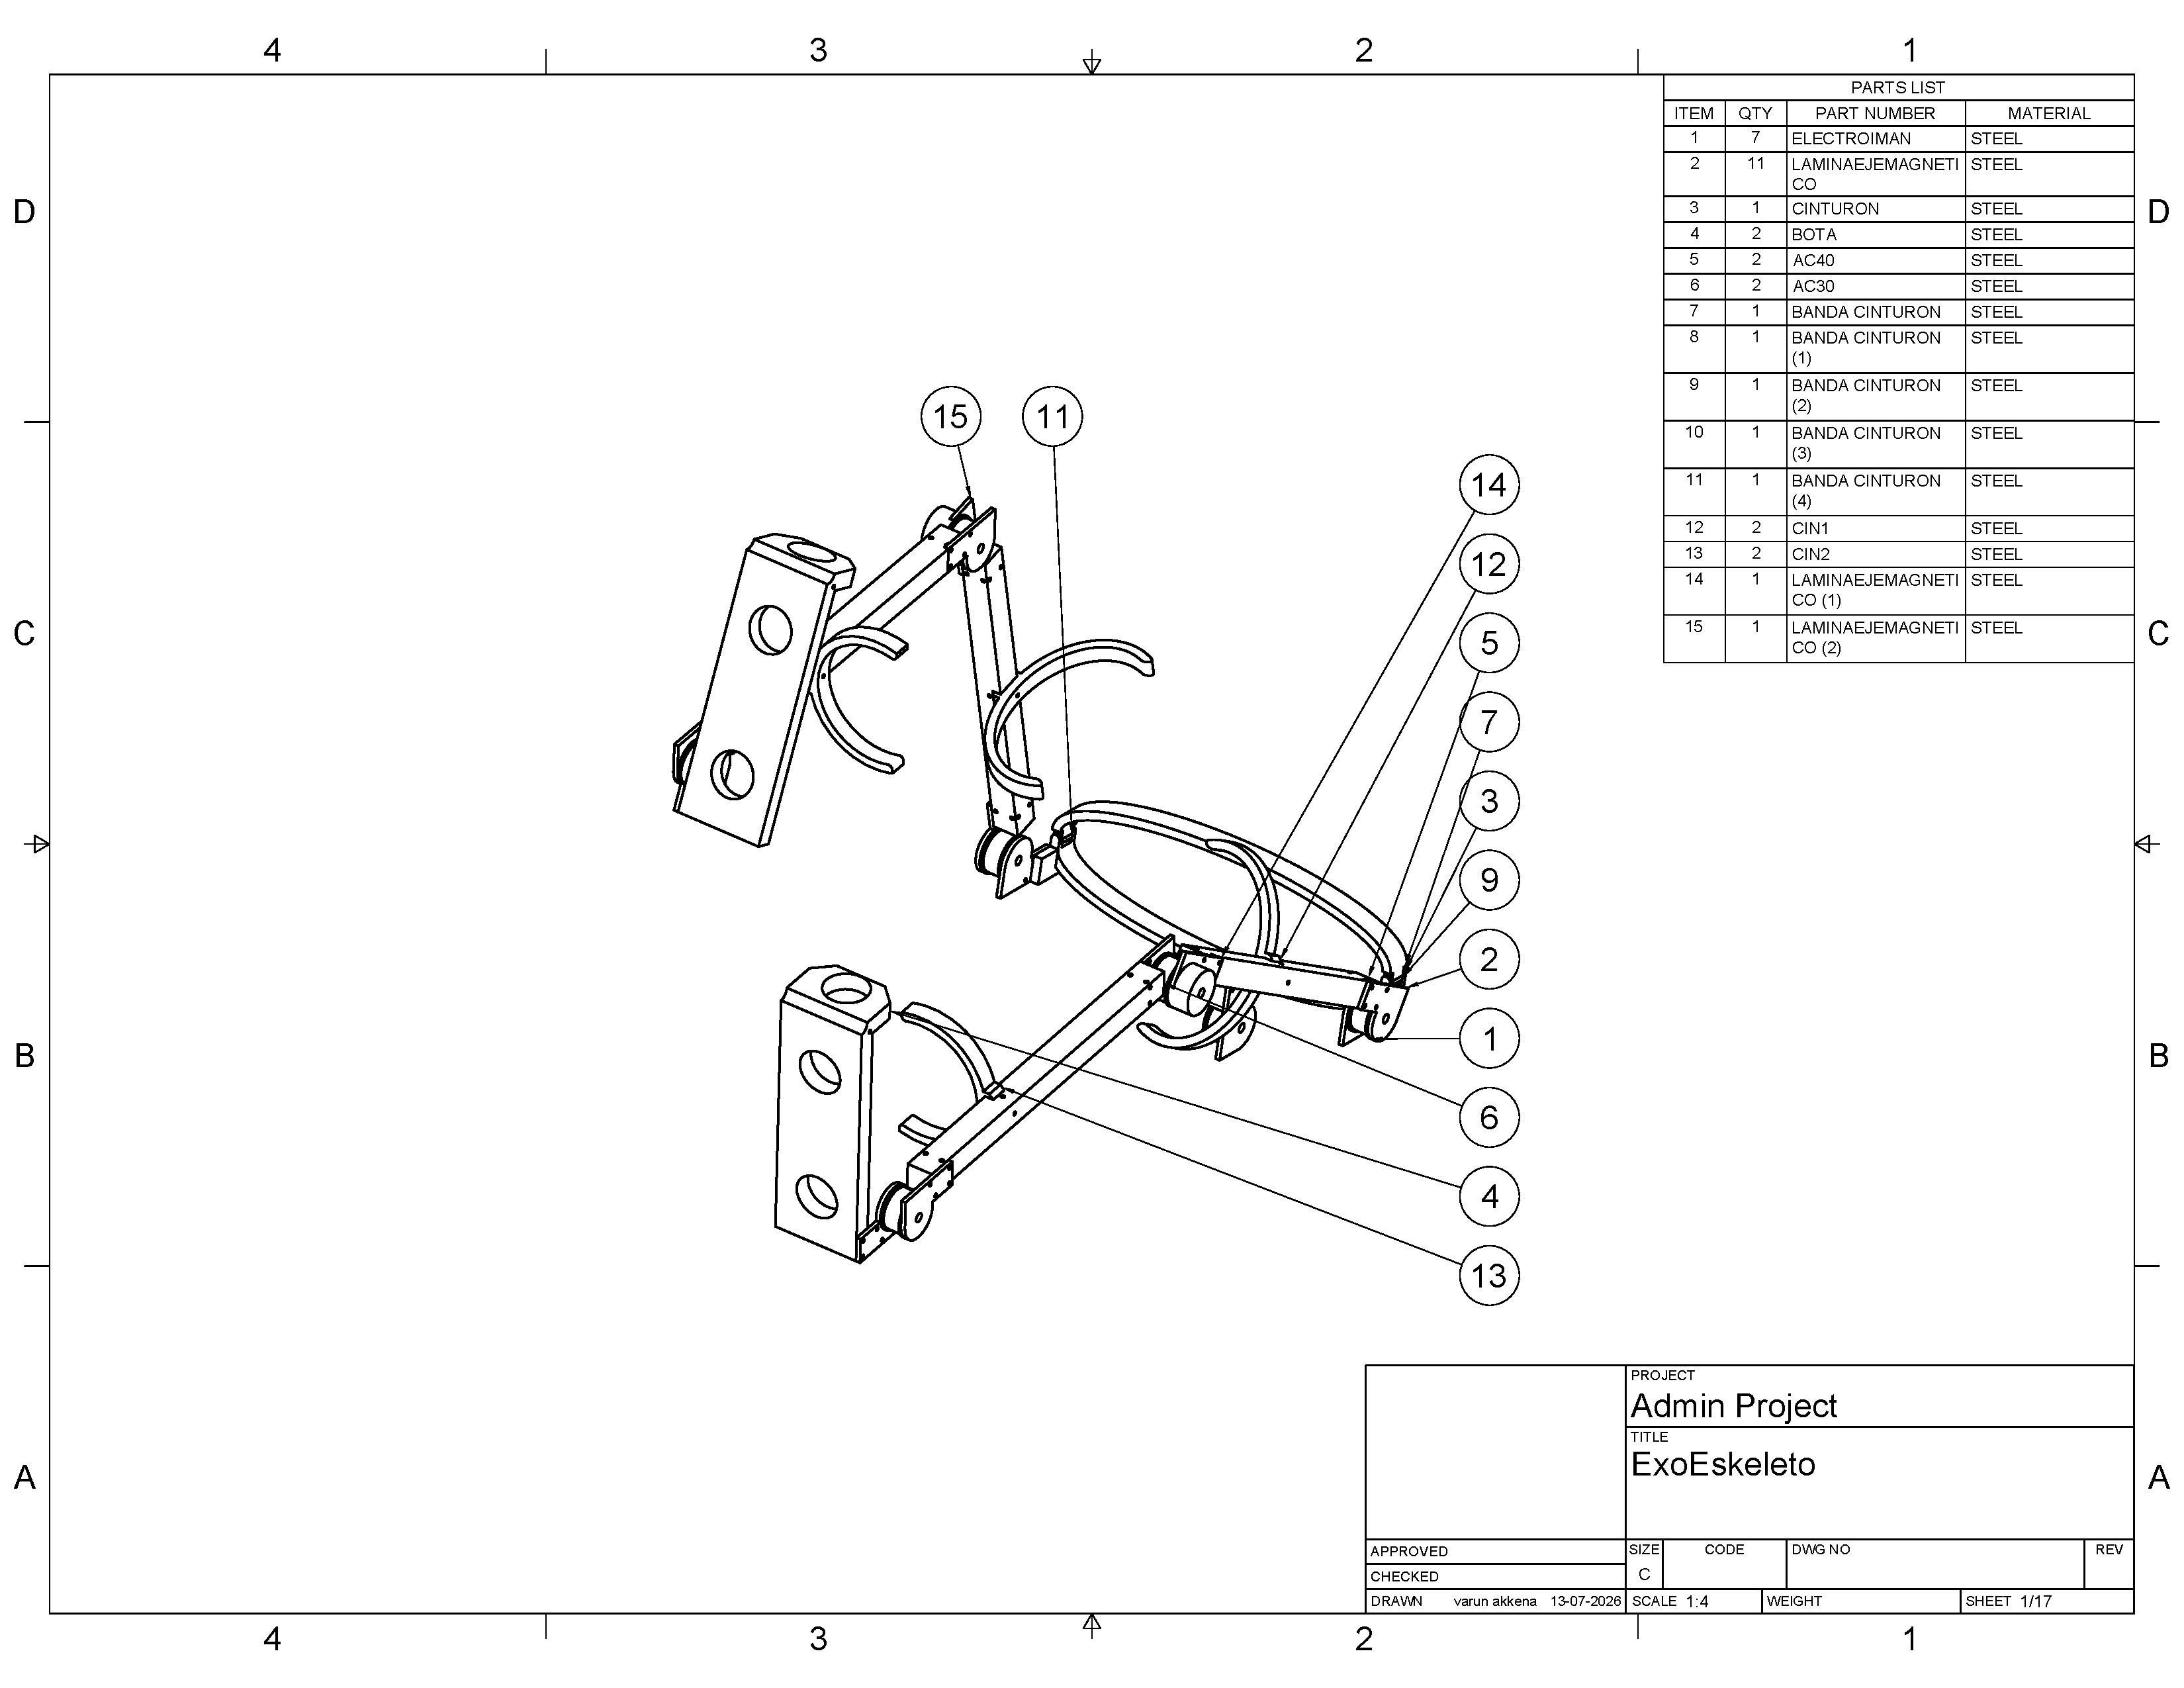
\includegraphics[page=1,width=0.65\linewidth,trim=27mm 31mm 27mm 28mm,clip]{ExoEskeleto Drawing v1.pdf}
  \end{center}

  \vspace{-2mm}
  \begin{center}
    \ratingcard{HIP}{120--150\Nm}{peak output, each side}\hfill
    \ratingcard{KNEE}{80--110\Nm}{peak output, each side}\hfill
    \ratingcard{ANKLE}{120--150\Nm}{peak output, each side}
  \end{center}
  \vspace{5mm}

  \begin{tabularx}{\linewidth}{@{}>{\bfseries\color{Navy}}p{35mm}X@{}}
    Source drawing & \texttt{ExoEskeleto Drawing v1.pdf}, 17 sheets \\
    Drawing date & 13 July 2026 \\
    Reference user & 80 kg \\
    Report status & Preliminary sizing; not approved for human testing \\
  \end{tabularx}

  \vfill
  {\small\color{Muted}Prepared from the geometry and bill of materials supplied in the source drawing.}
\end{titlepage}

\pagenumbering{arabic}

\highlightbox{Warm}{%
  \textbf{Scope and safety limitation.} This report is a first-pass actuator-sizing study based on the drawing and explicitly stated assumptions. It is not a final design approval or safety certification. Complete CAD mass-property extraction, multibody simulation, structural FEA, brake validation, thermal/electrical analysis, and controlled bench testing are required before testing on a person.
}

\tableofcontents
\vspace{4mm}

\section{Executive summary}

The 17-sheet drawing establishes the overall exoskeleton arrangement and principal link geometry. It does not define rotary motors, gearboxes, rated joint torques, component mass properties, actuator moment arms, gait profiles, or an assistance target. The bill of materials instead identifies seven electromagnets and eleven magnetic laminations or plates.

For a reference 80 kg user and a full lower-limb support envelope, the recommended preliminary output-side ratings are shown in Table~\ref{tab:ratings}. Six powered flexion/extension joints are implied if both hip, knee, and ankle joints are actuated.

Applying the Lagrange-Euler equation to the report's three-link reference model gives, for the stated horizontal dynamic example, $60.21\Nm$ and 90.31 W at the hip, $17.99\Nm$ and 35.98 W at the knee, and $2.54\Nm$ and 6.35 W at the ankle. These are unfactored swing-phase values for human-segment mass only; they exclude exoskeleton mass and ground-reaction force.

\begin{table}[H]
\centering
\caption{Preliminary joint-output design envelope, each side.}
\label{tab:ratings}
\small
\begin{tabularx}{\linewidth}{@{}>{\raggedright\arraybackslash}p{32mm}
  >{\centering\arraybackslash}p{24mm}
  >{\centering\arraybackslash}p{24mm}
  >{\centering\arraybackslash}p{19mm}X@{}}
\toprule
\textbf{Joint} & \textbf{Continuous torque} & \textbf{Peak torque} & \textbf{Output speed} & \textbf{Approximate actuator class} \\
\midrule
Hip flexion/extension & 45--60\Nm & 120--150\Nm & 0--3 rad/s & 300--500 W BLDC with low-backlash reducer \\
Knee flexion/extension & 30--45\Nm & 80--110\Nm & 0--4 rad/s & 250--400 W BLDC with low-backlash reducer \\
Ankle plantar/dorsiflexion & 45--60\Nm & 120--150\Nm & 0--5 rad/s & 350--600 W BLDC with reducer or remote transmission \\
\bottomrule
\end{tabularx}
\end{table}

\highlightbox{PaleTeal}{%
  \textbf{Primary design finding.} The electromagnets should be treated as auxiliary locks, clutches, or mode-selection devices unless their force-versus-gap and friction performance are demonstrated. They should not be assumed to replace torque-controlled rotary actuators or certified fail-safe brakes.
}

\section{Drawing basis and observed geometry}

\subsection{Information established by the drawing}

\begin{itemize}
  \item Overall envelope: approximately 1009 mm high, 1009 mm long, and 662 mm wide (sheet 2).
  \item Principal long members: approximately 400--420 mm on the detail sheets.
  \item Several circular joint/interface details: approximately 50 mm outside diameter with 10 mm bores.
  \item Bill of materials: seven \texttt{ELECTROIMAN} units and eleven magnetic laminations or plates.
  \item Listed structural parts are identified as steel.
  \item The assembly appears to comprise bilateral lower-limb links connected to a waist ring and foot/boot interfaces.
\end{itemize}

\subsection{Information not supplied}

The drawing does not provide maximum user mass, payload, part masses, centres of mass, gait cycle, required assistance percentage, motor torque-speed curves, gearbox ratios or efficiencies, bearing friction, joint range, structural steel grade, weld specifications, or electromagnet force data. These omissions prevent an exact CAD-derived actuator calculation.

\section{Reference design case}

The assumptions in Table~\ref{tab:assumptions} provide a transparent first-pass sizing case. Segment masses are anthropometric approximations and exclude exoskeleton hardware.

\begin{table}[H]
\centering
\caption{Reference assumptions used in the calculations.}
\label{tab:assumptions}
\begin{tabularx}{0.88\linewidth}{@{}X>{\raggedleft\arraybackslash}p{59mm}@{}}
\toprule
\textbf{Parameter} & \textbf{Assumption} \\
\midrule
User mass & 80 kg \\
Thigh length & 0.42 m \\
Shank length & 0.40 m \\
Foot COM distance from ankle & 0.13 m \\
One thigh mass & 10.0\% body mass = 8.00 kg \\
One shank mass & 4.65\% body mass = 3.72 kg \\
One foot mass & 1.45\% body mass = 1.16 kg \\
Thigh and shank COM location & 43.3\% of segment length from proximal joint \\
Gravity, $g$ & $9.81\unit{m/s^2}$ \\
Dynamic multiplier & 2.0 \\
Engineering factor after dynamics & 1.5 \\
\bottomrule
\end{tabularx}
\end{table}

The dynamic and engineering factors are included to establish an actuator selection envelope. Final load cases must instead use measured or simulated joint torque histories and include every moving exoskeleton component.

\section{Static gravity calculations}

For a point mass, the gravity moment about a joint is
\begin{equation}
  T = m g r,
\end{equation}
where $r$ is the horizontal distance from the joint axis. Gravity torque is largest when the segment is approximately horizontal.

\subsection{Hip: one leg held horizontal}

\begin{align}
T_{\mathrm{hip}} = g\big[&m_t(0.433L_t)
  + m_s(L_t+0.433L_s) \notag\\
  &+m_f(L_t+L_s+r_f)\big].
\end{align}

For the 80 kg reference user,
\begin{equation}
  \boxed{T_{\mathrm{hip}} = 46.7\Nm}
\end{equation}
for limb self-weight alone. This does not include the exoskeleton links, actuator masses, payload, or ground-reaction effects.

\subsection{Knee: shank and foot held horizontal}

\begin{equation}
T_{\mathrm{knee}} = g\left[m_s(0.433L_s)+m_f(L_s+r_f)\right],
\end{equation}
giving
\begin{equation}
  \boxed{T_{\mathrm{knee}} = 12.3\Nm}.
\end{equation}

\subsection{Ankle: ground-reaction load governs}

Foot self-weight produces only about $1.5\Nm$. This is not the governing ankle case. During standing and walking, ground-reaction force acts at a horizontal offset from the ankle. For the complete 80 kg body load and a 50--120 mm centre-of-pressure offset,
\begin{align}
T_{\mathrm{ankle}}
 &= (80)(9.81)(0.05\text{ to }0.12) \\
 &= \boxed{39\text{ to }94\Nm}.
\end{align}

In symmetric double support, each side may carry approximately half the load. In single support, one side can approach the full value and can exceed it dynamically.

\section{Lagrange-Euler torque and power calculation}

\subsection{Three-link planar model}

Let
\begin{equation}
  \mathbf q = [q_1\ q_2\ q_3]^T
\end{equation}
contain the relative hip, knee, and ankle angles. The pelvis is treated as a fixed base; $q_1$ is measured from the global horizontal, while $q_2$ and $q_3$ are relative angles. Positive rotation is counter-clockwise.

For the three moving segments, the kinetic and potential energies are
\begin{align}
K &= \frac{1}{2}\sum_{i=1}^{3}
  \left(m_i\dot{\mathbf r}_i^T\dot{\mathbf r}_i
  + I_i\omega_i^2\right),\\
V &= \sum_{i=1}^{3}m_i g y_i,
\end{align}
and the Lagrangian is $\mathcal L=K-V$. Applying the requested equation at each joint,
\begin{equation}
  \tau_i=\frac{d}{dt}\left(\frac{\partial\mathcal L}
  {\partial\dot q_i}\right)-\frac{\partial\mathcal L}{\partial q_i},
\end{equation}
gives the manipulator form
\begin{equation}
\boxed{\boldsymbol\tau_{\mathrm{act}}
=\mathbf M(\mathbf q)\ddot{\mathbf q}
+\mathbf C(\mathbf q,\dot{\mathbf q})\dot{\mathbf q}
+\mathbf G(\mathbf q)-\mathbf J_f^T\mathbf F_{\mathrm{ext}}.}
\end{equation}

The final term is essential in stance: $\mathbf F_{\mathrm{ext}}$ is the measured ground-reaction force at the foot and $\mathbf J_f$ is the foot Jacobian. It is set to zero in the numerical swing example because no force history is supplied.

Segment inertias are estimated using $I_i=m_i(k_iL_i)^2$. The radius-of-gyration fractions for thigh, shank, and foot are 0.323, 0.302, and 0.475, respectively. The calculation includes human segment mass only.

\subsection{Numerical input state}

The selected instant is deliberately explicit so that the result can be reproduced or replaced with measured data.

\begin{table}[H]
\centering
\caption{State used for the illustrative Lagrange-Euler calculation.}
\label{tab:lagrange-input}
\begin{tabular}{@{}lccc@{}}
\toprule
\textbf{Quantity} & \textbf{Hip} & \textbf{Knee} & \textbf{Ankle} \\
\midrule
$q_i$ & $0^\circ$ & $0^\circ$ & $0^\circ$ \\
$\dot q_i$ & 1.5 rad/s & 2.0 rad/s & 2.5 rad/s \\
$\ddot q_i$ & $3.0\unit{rad/s^2}$ & $4.0\unit{rad/s^2}$ & $5.0\unit{rad/s^2}$ \\
External foot force & \multicolumn{3}{c}{$\mathbf F_{\mathrm{ext}}=[0\ 0]^T\unit{N}$} \\
\bottomrule
\end{tabular}
\end{table}

At this collinear horizontal configuration,
\begin{equation}
\mathbf M=
\begin{bmatrix}
2.8397 & 1.0382 & 0.1610\\
1.0382 & 0.5094 & 0.0976\\
0.1610 & 0.0976 & 0.0373
\end{bmatrix}\unit{kg\,m^2},
\end{equation}
\begin{equation}
\mathbf G=
\begin{bmatrix}46.7308\\12.3518\\1.4793\end{bmatrix}\Nm,
\qquad
\mathbf C\dot{\mathbf q}=\mathbf 0.
\end{equation}

The Coriolis/centrifugal vector is zero at this particular collinear state because the required sine coupling terms vanish; it is generally non-zero at other postures.

\subsection{Calculated torque and joint power}

Instantaneous joint mechanical power is
\begin{equation}
  \boxed{P_i=\tau_i\dot q_i.}
\end{equation}
Positive power drives the motion; negative power indicates braking or potential regeneration.

\begin{table}[H]
\centering
\caption{Unfactored dynamic result for the state in Table~\ref{tab:lagrange-input}.}
\label{tab:lagrange-result}
\small
\begin{tabular}{@{}lrrrr@{}}
\toprule
\textbf{Joint} & \textbf{Inertial} & \textbf{Gravity} & \textbf{Total torque} & \textbf{Joint power} \\
& \textbf{(N m)} & \textbf{(N m)} & \textbf{(N m)} & \textbf{(W)} \\
\midrule
Hip & 13.477 & 46.731 & \textbf{60.208} & \textbf{90.311} \\
Knee & 5.640 & 12.352 & \textbf{17.992} & \textbf{35.985} \\
Ankle & 1.060 & 1.479 & \textbf{2.539} & \textbf{6.348} \\
\midrule
Total & & & & \textbf{132.644} \\
\bottomrule
\end{tabular}
\end{table}

For example, the first-joint calculation is
\begin{align}
\tau_1 &=
  2.8397(3)+1.0382(4)+0.1610(5)+46.7308 \\
  &=\boxed{60.208\Nm},\\
P_1 &= \tau_1\dot q_1
  =60.208(1.5)=\boxed{90.311\unit{W}}.
\end{align}

If a separate 1.5 engineering factor is applied after this trajectory calculation, the resulting provisional values are 90.31, 26.99, and $3.81\Nm$ for hip, knee, and ankle. The ankle value remains unsuitable for stance sizing because the ground-reaction term is absent.

\subsection{Illustrative gearbox mapping}

Using 80:1 hip and knee reducers, a 60:1 ankle reducer, and 75\% gearbox efficiency gives Table~\ref{tab:motor-map}. Shaft power is joint power divided by gearbox efficiency; electrical input will be higher again after motor and drive losses.

\begin{table}[H]
\centering
\caption{Motor-side result for the illustrative swing state.}
\label{tab:motor-map}
\begin{tabular}{@{}lrrrr@{}}
\toprule
\textbf{Joint} & \textbf{Ratio} & \textbf{Motor torque} & \textbf{Motor speed} & \textbf{Shaft power} \\
& & \textbf{(N m)} & \textbf{(rpm)} & \textbf{(W)} \\
\midrule
Hip & 80:1 & 1.003 & 1146 & 120.4 \\
Knee & 80:1 & 0.300 & 1528 & 48.0 \\
Ankle & 60:1 & 0.056 & 1432 & 8.5 \\
\bottomrule
\end{tabular}
\end{table}

As a conservative instantaneous envelope, multiplying the preliminary peak torque and maximum speed in Table~\ref{tab:ratings} gives 450 W at the hip, 440 W at the knee, and 750 W at the ankle. Torque and speed peaks normally occur at different times, so these products are upper bounds rather than continuous motor ratings. Final continuous power must be based on cycle RMS torque, measured speed histories, gearbox efficiency maps, and thermal limits.

\section{Motor and transmission sizing}

\subsection{Torque and ratio relationship}

For gearbox ratio $N$ and transmission efficiency $\eta$, required motor torque is
\begin{equation}
  T_{\mathrm{motor}}=\frac{T_{\mathrm{joint}}}{N\eta}.
\end{equation}

For a $120\Nm$ peak joint, an 80:1 ratio, and 75\% efficiency,
\begin{equation}
  T_{\mathrm{motor,peak}}
  =\frac{120}{80(0.75)}
  =\boxed{2.0\Nm}.
\end{equation}

At 60:1 and 80\% efficiency, the same joint requires $2.5\Nm$ motor peak torque. A reduction range near 50:1--100:1 is a reasonable starting point, but the final ratio must satisfy joint torque, joint speed, thermal duty, backlash, and backdrivability requirements simultaneously.

\subsection{Recommended architecture}

\begin{itemize}
  \item 48 V BLDC or PMSM actuators to limit current and cable mass.
  \item Absolute joint encoder plus motor encoder.
  \item Low-backlash harmonic, cycloidal, or well-supported planetary reducer.
  \item Torque sensing through a strain element or series-elastic element.
  \item Normally engaged mechanical brake at each load-bearing joint.
  \item Mechanical hard stops independent of software.
\end{itemize}

High reduction improves torque density but reduces backdrivability and increases reflected inertia. Torque sensing and mechanical compliance are strongly preferred for a wearable device. Distal motor mass also increases swing torque; proximal knee actuation and remote ankle transmission should be evaluated.

\subsection{Scaling and partial assistance}

For a user mass $M$ different from 80 kg, a first approximation is
\begin{equation}
T_{\mathrm{new}} = T_{\mathrm{table}}\left(\frac{M}{80}\right)
+T_{\mathrm{exo+payload}}.
\end{equation}

For partial assistance, multiply the biological joint-torque target by the desired assistance fraction. For example, 40\% assistance at a $150\Nm$ ankle peak requires approximately $60\Nm$ actuator output before transmission losses and friction are added.

\section{Electromagnet feasibility check}

If an electromagnet at a nominal 50 mm diameter interface is expected to resist joint torque through friction at an effective radius of approximately 25 mm, the required tangential force is
\begin{equation}
  F_t=\frac{T}{r}.
\end{equation}

\begin{table}[H]
\centering
\caption{Tangential force implied at a 25 mm effective radius.}
\begin{tabular}{@{}rr@{}}
\toprule
\textbf{Joint torque} & \textbf{Tangential force} \\
\midrule
$60\Nm$ & 2400 N \\
$120\Nm$ & 4800 N \\
$150\Nm$ & 6000 N \\
\bottomrule
\end{tabular}
\end{table}

Friction torque is $T=\mu F_n r$. With a nominal dry friction coefficient of 0.3, holding $120\Nm$ at a 25 mm radius requires
\begin{equation}
F_n=\frac{120}{0.3(0.025)}=\boxed{16{,}000\unit{N}}
\end{equation}
of magnetic normal force. Air gaps, surface contamination, coil heating, and loss of electrical power further reduce dependable holding capacity.

\highlightbox{Warm}{%
  \textbf{Design implication.} Do not use the drawn electromagnets as the sole load-bearing joint brakes without a demonstrated force/torque test. If used for locking or mode selection, add a mechanically positive, normally locked feature so that loss of power cannot release the user.
}

\section{Structural and integration observations}

\begin{itemize}
  \item Several details show 10 mm bores. A pin at this interface requires combined shear, bearing, bending, fatigue, and retention analysis; bore diameter alone is insufficient.
  \item Long 400--420 mm links and offset cuffs introduce bending and torsion in addition to in-plane joint torque.
  \item The BOM states steel but does not provide grade, complete thickness data, heat treatment, weld details, or allowable stress.
  \item Joint axes must align with the user's anatomical hip, knee, and ankle axes. Misalignment can create harmful cuff forces even when motor torque is within its limit.
  \item Knee motors should preferably be placed proximally. The ankle may benefit from cable, Bowden, belt, or linkage transmission to reduce distal mass.
  \item Motor torque must not be the only protection against collapse during power loss.
\end{itemize}

\clearpage
\section{Data required for final sizing}

\begin{enumerate}
  \item Maximum user mass and carried payload.
  \item Intended function: rehabilitation assistance, full weight support, sit-to-stand, walking, or static locking.
  \item Required degrees of freedom, angular limits, and mechanical stop positions.
  \item Target gait speed and joint angle, velocity, and acceleration profiles versus time.
  \item CAD mass and centre of mass for each link, motor, gearbox, battery, and attachment.
  \item Electromagnet model, force-versus-gap curve, coil power, friction material, effective radius, and fail-safe behaviour.
  \item Gearbox ratio, efficiency, backlash, rated output moment, shock rating, and life.
  \item Ground-reaction-force cases and required assistance percentage.
\end{enumerate}

\section{Conclusion}

For an 80 kg reference user and full lower-limb support, size each side initially for $120$--$150\Nm$ peak at the hip, $80$--$110\Nm$ peak at the knee, and $120$--$150\Nm$ peak at the ankle, with the continuous ratings in Table~\ref{tab:ratings}. These are output-side design-envelope values, not motor-shaft values.

The seven electromagnets identified in the drawing are best treated as auxiliary locks or clutches. They are not substitutes for torque-controlled rotary motors or validated fail-safe brakes. Human testing should not begin until the missing design inputs are resolved and the system has passed simulation, structural verification, brake testing, thermal analysis, electrical safety review, and controlled bench trials.

\vfill
\highlightbox{PaleBlue}{%
  \textbf{Next engineering release.} Replace the reference anthropometric model with CAD mass properties and measured motion/load cases, then issue a joint-by-joint motor, reducer, brake, bearing, pin, and controller specification.
}

\end{document}
